%%
%% Generated by gpt_translate from test/images.tex, on 2024-07-09 16:43:18 using model gpt-3.5-turbo-16k
%%

% GPT CHUNK%
\documentclass{ximera}
../preamble.tex
\addPrintStyle{..}

\begin{document}
    \xmtitle{TikZ pictures}{}

    \providecommand{\psize}[1]{
        \pgfmathparse{#1}
        \pgfmathresult pt
    }
    
    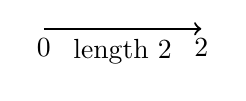
\begin{tikzpicture}
        \draw[thick,->]
        (0,0) node[below] {$0$} 
        --  node[below] {length 2}
        (2,0) node[below] {$2$};
    \end{tikzpicture}
    , a tikzpicture without anything else.

    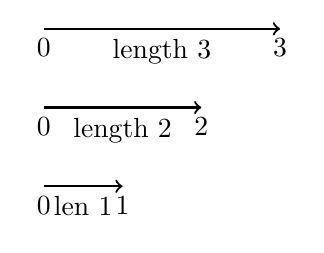
\begin{tikzpicture}
        \draw[yshift=0cm, thick,->] (0,0) node[below] {$0$}  --  node[below] {len    1} (1,0) node[below] {$1$};
        \draw[yshift=1cm, thick,->] (0,0) node[below] {$0$}  --  node[below] {length 2} (2,0) node[below] {$2$};
        \draw[yshift=2cm, thick,->] (0,0) node[below] {$0$}  --  node[below] {length 3} (3,0) node[below] {$3$};
    \end{tikzpicture}
    , a tikzpicture with several lengths.

    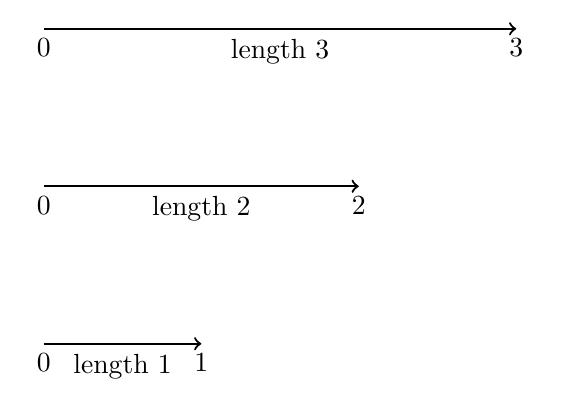
\begin{tikzpicture}[scale=2]
        \draw[yshift=0cm, thick,->] (0,0) node[below] {$0$}  --  node[below] {length 1} (1,0) node[below] {$1$};
        \draw[yshift=1cm, thick,->] (0,0) node[below] {$0$}  --  node[below] {length 2} (2,0) node[below] {$2$};
        \draw[yshift=2cm, thick,->] (0,0) node[below] {$0$}  --  node[below] {length 3} (3,0) node[below] {$3$};
    \end{tikzpicture}
    , a tikzpicture with scale=2.

    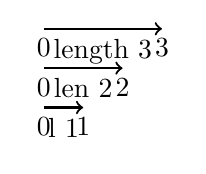
\begin{tikzpicture}[scale=0.5]
        \draw[yshift=0cm, thick,->] (0,0) node[below] {$0$}  --  node[below] {l      1} (1,0) node[below] {$1$};
        \draw[yshift=1cm, thick,->] (0,0) node[below] {$0$}  --  node[below] {len    2} (2,0) node[below] {$2$};
        \draw[yshift=2cm, thick,->] (0,0) node[below] {$0$}  --  node[below] {length 3} (3,0) node[below] {$3$};
    \end{tikzpicture}
    , a tikzpicture with scale=0.5.

    A tikzpicture inside a \verb|\begin{image}[\textwidth]| with size =\psize{\textwidth} (and textwidth =\the\textwidth).
    \begin{image}[\textwidth]
        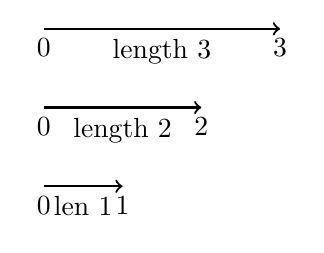
\begin{tikzpicture}
            \draw[yshift=0cm, thick,->] (0,0) node[below] {$0$}  --  node[below] {len    1} (1,0) node[below] {$1$};
            \draw[yshift=1cm, thick,->] (0,0) node[below] {$0$}  --  node[below] {length 2} (2,0) node[below] {$2$};
            \draw[yshift=2cm, thick,->] (0,0) node[below] {$0$}  --  node[below] {length 3} (3,0) node[below] {$3$};
            \end{tikzpicture}
    \end{image}
    A tikzpicture inside a \verb|\begin{image}[0.5\textwidth]| with size =\psize{\textwidth} (and textwidth =\the\textwidth).
    \begin{image}[0.5\textwidth]
        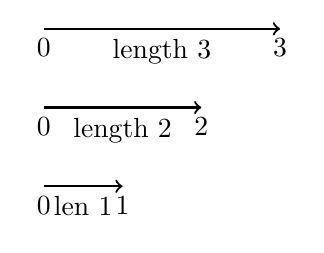
\begin{tikzpicture}
            \draw[yshift=0cm, thick,->] (0,0) node[below] {$0$}  --  node[below] {len    1} (1,0) node[below] {$1$};
            \draw[yshift=1cm, thick,->] (0,0) node[below] {$0$}  --  node[below] {length 2} (2,0) node[below] {$2$};
            \draw[yshift=2cm, thick,->] (0,0) node[below] {$0$}  --  node[below] {length 3} (3,0) node[below] {$3$};
            \end{tikzpicture}
    \end{image}

    A tikzpicture inside a \verb|\begin{image}[5cm]| with size =\psize{\textwidth} (and textwidth =\the\textwidth).
    \begin{image}[5cm]
        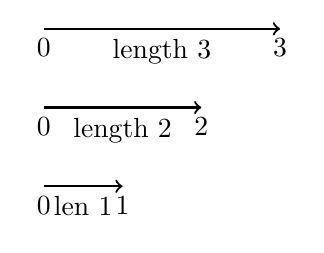
\begin{tikzpicture}
            \draw[yshift=0cm, thick,->] (0,0) node[below] {$0$}  --  node[below] {len    1} (1,0) node[below] {$1$};
            \draw[yshift=1cm, thick,->] (0,0) node[below] {$0$}  --  node[below] {length 2} (2,0) node[below] {$2$};
            \draw[yshift=2cm, thick,->] (0,0) node[below] {$0$}  --  node[below] {length 3} (3,0) node[below] {$3$};
            \end{tikzpicture}
    \end{image}

    \end{document}